\section{Kedvezmények}


\newcounter{Kecounter}
\newcommand{\sorSzamKe}{\stepcounter{Kecounter}\theKecounter}

Amennyiben az ügyfél hozzájárul a számára elvégzett munka referenciának történő felhasználásához különböző mértékű árengedményekhez juthat.

\subsection{Kedvezményszintek}
A kedvezmények különböző szintekbe sorolhatók (\kovAzon{Ke\_\sorSzamKe}). Minden szinten a kivitelező megadhatja
a kedvezmény méretét (százalékban) az alkalmazás által megszabott intervallumon belül (pl. 5 - 10\%), amennyiben az adott munkánál fel kívánja ajánlani annak lehetőségét (\kovAzon{Ke\_\sorSzamKe}). 
A kedvezmény ezen korlátozása segíti az ügyfelek szakemberek általi bármiféle átverésének, vagy félrevezetésének elkerülését, akár legyen ez túl alacsony kedvezmény egy részletes referenciáért, vagy félrevezetően nagy kedvezmények, ahol valójában a kezdeti ár túl magas, és nem tükrözi a valós piaci viszonyokat.

Az összes kedvezmény szintre vonatkozik, hogy az ügyfél előzetesen hozzájárul a vállalt feltételek teljesítésére, azzal a megkötéssel, hogy minden médiaanyagot mely a kivitelezéssel kapcsolatban készült, kizárólag az oldalon történő üzletszerzés céljából használhatnak fel a szakemberek munkájuk minőségének bizonyítására (\kovAzon{Ke\_\sorSzamKe}).

\subsubsection{1. szint (0 - 3\%) – Megemlítés, értékelés, egy-két fotó} 
Az ügyfél hozzájárulásával lehetőséget biztosít a kivitelező számára, hogy a kész munkáról képeket készítsen. Ez a referencia segíti a kivitelezőt a szakmai portfóliója bővítésében és a leendő ügyfelek tájékoztatásában. A hozzájárulásért cserébe az ügyfél a kivitelező által előre meghatározott mértékű kedvezményben részesül, amely a szolgáltatás árából kerül levonásra.

\subsubsection{2. szint (3 - 5\%) – Négy-öt fotó, beltéri kép} 
Az ügyfél az első szint tartalmán túl ahhoz is hozzájárul, hogy a kész munkáról részletesebb, legalább négy-öt fotó készüljön és szerepelhessen benne az ingatlan beltere is, amennyiben ez releváns az adott munka szempontjából. Ez lehetőséget ad a kivitelező számára, hogy munkáját részletesebben dokumentálja és bemutassa. A további képek készítéséért cserébe az ügyfél magasabb szintű kedvezményben részesül.

\subsubsection{3. szint (5 - 8\%) – Videó} 
A második szint tartalmán felül az ügyfél hozzájárul ahhoz, hogy a kész munkáról videók készüljenek. A videók segítségével az elvégzett munka dinamikusabb, részletesebb módon kerül bemutatásra, ami tovább erősíti a kivitelező szakmai portfólióját. A videók készítéséhez való hozzájárulásért az ügyfél jelentősebb kedvezményben részesül.

\subsubsection{4. szint (8 - 10\%) – Kültéri és beltéri videós körbevezetés, pontos leírás} 
Az előző szinteken megfogalmazottak mellett az ügyfél hozzájárul ahhoz is, hogy a kivitelező kültéri és beltéri videós bemutatót készítsen, amely pontos leírással egészül ki. Ez a részletes dokumentáció lehetővé teszi az elvégzett munka mélyebb bemutatását, elősegítve a kivitelező további referenciáinak kiemelkedő minőségét. A videók jóváhagyásáért az ügyfél a szolgáltatás árából még nagyobb mértékű kedvezményben részesül.

\subsubsection{5. szint (10 - 15\%) – Személyes bemutatás} 
A negyedik szinten felül az ügyfél hozzájárul ahhoz is, hogy a kivitelező személyes bemutatót tarthasson a kész munkáról, előre egyeztetett időpontban. Ezek a bemutatók kizárólag referencia célját szolgálják, és segítik a kivitelezőt abban, hogy munkáját potenciális ügyfelek számára a helyszínen is megmutathassa.

A bemutatók lebonyolítására egy felső időkorlát kerül meghatározásra, amely legfeljebb 8 bemutatóórát tesz lehetővé, legfeljebb hat hónap időtartamra. Az ügyfél vállalja, hogy legalább 3 alkalommal biztosítja a bemutatóhoz szükséges lehetőséget, havonta legalább egy lehetséges időpontot garantálva. A személyes bemutató lehetőségéért az ügyfél a legmagasabb szintű kedvezményben részesül.

\subsection{A kedvezmény alkalmazásának menete}
Amennyiben az adott kivitelező munkájához megadja az árengedmény lehetőségét és az azokhoz szükséges vállalásokat,
az ügyfél a webes felületen dönthet, hogy él-e a lehetőséggel és kiválaszthatja annak szintjét (\kovAzon{Ke\_\sorSzamKe}).
Ezt követően a kedvezmény mértéke és az ezért cserébe vállalt feltételek a szerződésben rögzítésre kerülnek.

\subsection{A kedvezményrendszer használatának ösztönzése}
A kedvezményrendszerbe való csatlakozás nem kötelező a kivitelezők számára, erre a saját referenciájuk felállítása mellett más ösztönző tényezők is szóba jönnek:
\begin{itemize}
\item Sok referencia esetén magasabb prioritás kereséseknél (\kovAzon{Ke\_\sorSzamKe})
\item Engedmény az oldal használatáért fizetendő közvetítői díjból (\kovAzon{Ke\_\sorSzamKe})
\item Kiemelt partnerré válás lehetősége, ajánlás a webalkalmazás kezdőlapján (\kovAzon{Ke\_\sorSzamKe}).
\end{itemize} 

\begin{figure}[h]
	\centering
	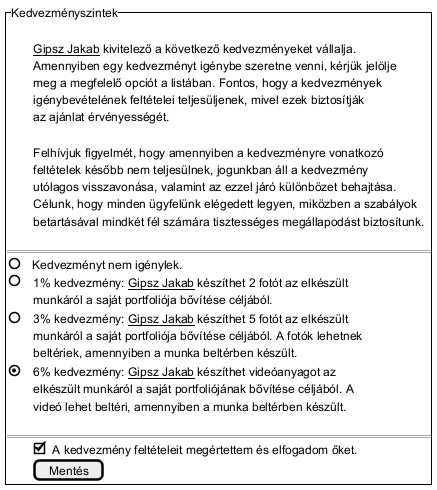
\includegraphics[scale=0.7]{img/kedvezmeny.png}
	\caption*{Kedvezmény igénylés}
	\label{fig:kedvez}
\end{figure}